% vim: set textwidth=78 autoindent:

\section{Lavorare con i dati raster}\label{label_raster}
\index{layer raster}

% when the revision of a section has been finalized, 
% comment out the following line:
%\updatedisclaimer

Questa Sezione descrive come visualizzare ed impostare le proprietà dei dati
raster. I formati raster attualmente supportati in QGIS includono:\index{layer raster!formato dati}

\begin{itemize}
\item Arc/Info Binary Grid
\item Arc/Info ASCII Grid
\item GRASS Raster
\item GeoTIFF
\item JPEG
\item Spatial Data Transfer Standard Grids (con alcune limitazioni)
\item USGS ASCII DEM
\item Erdas Imagine
\end{itemize}

Considerato che il supporto ai raster in QGIS è fornito dalla libreria GDAL,
oltre a quelli elencati è possibile che sia possibile caricare anche altri
formati supportati da GDAL - nel dubbio è comunuque possibile provare ad aprire il file
in QGIS per verificare l'esito. Ulteriori dettagli sono forniti all'Appendice \ref{appdx_gdal}
\index{layer raster!implementazione GDAL} o all'indirizzo
\url{http://www.gdal.org/formats_list.html}. Per caricare dati raster di
GRASS, fare riferimento alla Sezione~\ref{sec:load_grassdata}.

\subsection{Cosa sono i dati raster?}\label{label_whatsraster}
\index{layer raster!definizione}

I dati raster nei GIS sono matrici di celle discrete che rappresentano le
caratteristiche della superficie terrestre o dell'ambiente al di sopra o al di sotto
di essa. Ogni cella nella matrice raster presenta lo stesso formato e le celle
sono solitamente rettangolari (in QGIS saranno sempre rettangolari). Esempi
tipici di dati raster sono quelli provenienti dal telerilevamento come le
fotografie aeree o immagini proveniente dal satellite e dati
modellistici quali matrici dell’altitudine.

Diversamente dai dati vettoriali, i dati raster di solito non hanno associato
un database contenente i dati descrittivi di ogni cella.

I dati raster, infine, sono geocodificati in base alla risoluzione del pixel e
alle coordinate x/y di un angolo del raster che ne consente un corretto
posizionamento nella vista mappa. 

QGIS utilizza le informazioni di georeferenziazione incorporate nel layer
raster (ad es. GeoTiff) o in un apposito "world file" per visualizzare
correttamente i dati.\index{layer raster!georeferenziazione}
	
\subsection{Caricamento dati raster in QGIS}\label{label_loadraster}

I layer raster possono essere caricati sia selezionando nella barra lo
strumento \toolbtntwo{mActionAddRasterLayer}{Aggiungi layer raster} o
scegliendo la voce di menu
\mainmenuopt{Layer}>\dropmenuopttwo{mActionAddRasterLayer}{Aggiungi layer
raster}. È possibile caricare più di un layer alla volta tenendo premuto il
tasto \keystroke{Control} o \keystroke{Shift} mentre si effettua la selezione
multipla con il mouse sui layer nella finestra di dialogo \dialog{Apre
unraster supportato da GDAL}.\index{layer raster!caricamento}

Quando il layer è caricato è possibile cliccare nella legenda sul relativo
nome con il tasto destro per selezionare ed attivare opzioni specifiche o per
aprire la finestra per l'impostazione delle proprietà del layer raster.

\minisec{Menu contestuale per layer raster}

\begin{itemize}
\item \dropmenuopt{Zoom all'estensione del layer}
\item \dropmenuopt{Zoom alla scala migliore (100\%)}
\item \dropmenuopt{Aggiungi alla panoramica}
\item \dropmenuopt{Rimuovi}
\item \dropmenuopt{Proprietà}
\item \dropmenuopt{Rinomina}
\item \dropmenuopt{Aggiungi gruppo}
\item \dropmenuopt{Espandi tutto}
\item \dropmenuopt{Comprimi tutto}
\item \dropmenuopt{Mostra gruppi}
\end{itemize}
	
\subsection{Finestra delle proprietà raster}\label{label_rasterprop}

Per visualizzare ed impostare le proprietà di un layer raster, fare doppio
click sul nome del raster nella legenda o cliccare su di esso con il tasto
destro e scegliere \dropmenuopt{Proprietà} dal menu contestuale:\index{layer raster!menu contestuale}
La figura \ref{fig:raster_properties} mostra la finestra \dialog{Proprietà raster}. 
Ci sono diverse schede nella finestra: 

\begin{itemize}
 \item \tab{Simbologia}
 \item \tab{Trasparenza}
 \item \tab{Mappa colore}
 \item \tab{Generale}
 \item \tab{Metadata}
 \item \tab{Piramidali}
 \item \tab{Istogramma}
\end{itemize}

\begin{figure}[h]
  \begin{center}
   \caption{Finestra delle proprietà dei layer raster \nixcaption}\label{fig:raster_properties}\smallskip
   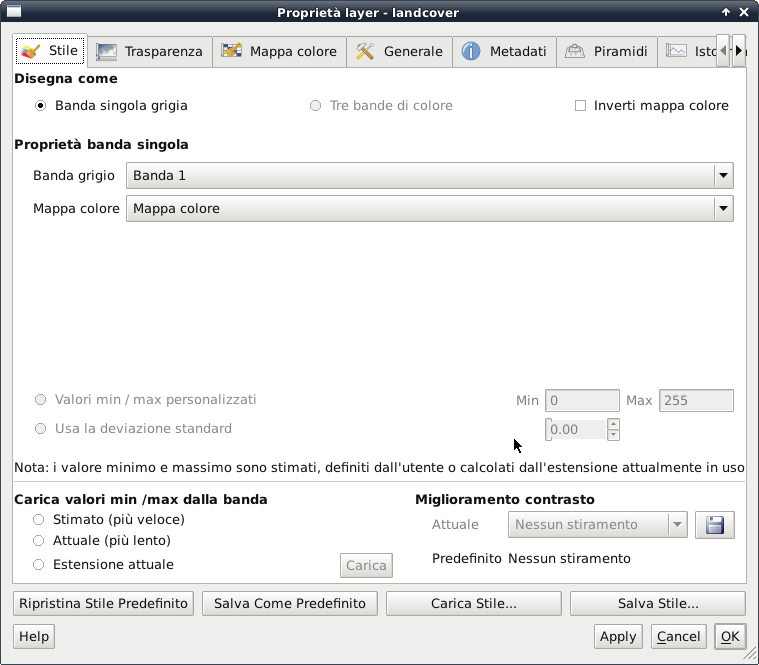
\includegraphics[clip=true, width=14cm]{rasterPropertiesDialog}
\end{center}  
\end{figure}

\subsubsection{Scheda Simbologia}\label{label_sombology}

QGIS può rendere a video i raster in due modi:\index{layer raster!canali supportati}

\begin{itemize}
\item Banda singola grigia - viene campionata una sola banda dell'immagine e
resa in gradazioni di grigio o in pseudocolore.
\item Tre bande di colore - vengono rese a video tre bande dell'immagine
ognuna rappresentante le componenti rosso, verde o blu che saranno composte
per creare un'immagine a colori.
\end{itemize}

È possibile invertire i colori in modo che i colori chiari divengano scuri e
viceversa selezionando la casella di controllo \checkbox{Inverti mappa colore}.

\minisec{Resa in banda singola}

Selezionando questa opzione vengono offerte due possibilità tra le quali
scegliere. Innanzitutto se il layer è multibanda è possibile scegliere quale
banda si desidera venga impiegata per la resa a video. 

La seconda opzione offre una selezione di tabelle colori preimpostate per la
resa a video.

Le scelte possibili disponibili nel menu a tendina sono
\selectstring{Mappa colore}{Scala di grigi}, impostazione di default.
Altre scelte possibili sono
\begin{itemize}
\item Pseudo colore
\item Freak Out
\item Mappa colore
\end{itemize}

Quando viene selezionata l'opzione \selectstring{Mappa colore}{Mappa colore},
viene abilitata la scheda \tab{Mappa colore}. Si vedano ulteriori
informazioni al capitolo \ref{label_colormaptab}.

Per immagini in pseudocolore in QGIS è possibile limitare i dati visualizzati
per mostrare soltanto le celle i cui valori ricadono all'interno di una deviazione standard
definita.\index{layer raster!deviazione standard} Ciò può essere utile quando
nella griglia raster si hanno una o due celle con valori anormalmente alti
che hanno un impatto negativo sulla resa a video del raster.

\minisec{Resa in tre bande}

Questa opzione offre un considerevole numero di possibilità di modifica
dell'aspetto del raster. Ad esempio è possibile cambiare il normale ordine RGB
delle bande e/o applicare una scala di colori in base ai valori min/max del
raster.

\begin{Tip}\caption{\textsc{Vedere una singola banda di un raster multibanda}}
\qgistip{Il modo corretto di visualizzare ad es. la sola banda rossa di
un'immagine multibanda non è quello di impostare le bande verde e blu a "Non
impostato", ma di impostare il tipo di immagine come scala di grigi e quindi
scegliere il rosso come banda da usare per il grigio.}
\end{Tip} 

\subsubsection{Scheda Trasparenza} \label{rastertab:transparency}

Questa scheda consente di impostare in QGIS un diverso grado di trasparenza per ogni layer raster.\index{layer raster!trasparenza}
Per settare una \guiheading{Trasparenza globale}, impostare il cursore a scorrimento al livello di trasparenza desiderato
in maniera tale da consentire la visualizzazione degli eventuali layer sottostanti. 
L'uso di questa impostazione può essere molto utile nei casi in cui si
desideri sovrapporre ad es. ad una mappa delle ombreggiature del rilievo (shaded
relief-map) assieme a una mappa raster contenente delle classificazioni, così da dare un
aspetto tridimensionale a quest'ultima.

La sezione \guiheading{Nessun valore} consente invece di definire la trasparenza per un certo valore del raster, che sarà quindi letto come un campo privo di dati del tipo {\em NODATA}. Di
conseguenza in corrispondenza di tutte le celle del raster contenenti quel
valore non verrà reso a video niente, determinando quindi una trasparenza per
il valore specificato.

È possibile definire la trasparenza in maniera ancora più dettagliata e
personalizzata nelle Sezione \guiheading{Opzioni di trasparenza
personalizzate}, nella quale è possibile impostare il grado di trasparenza per
ogni valore del raster.
Ad esempio se si volesse utilizzare quest'ultima sezione per visualizzare l'acqua del raster di esempio \filename{landcover.tif}
con una trasparenza del 20\%, bisognerà seguire la seguente procedura:

\begin{enumerate}
 \item Caricare il raster \filename{landcover}
 \item Aprire la finestra di dialogo \dialog{Proprietà} facendo doppio click
 sul nome del file nella legenda o cliccando su di esso con il tasto destro e
 scegliendo \dropmenuopt{Proprietà} dal menu contestuale
 \item Selezionare la scheda \tab{Trasparenza}
 \item \label{enum:add} Cliccare sul pulsante
 \toolbtntwo{mActionNewAttribute}{Aggiungi un valore manualmente}. Nella lista
 pixel apparirà una nuova riga
 \item \label{enum:transp} Inserire il valore del raster per il quale si
 desidera modificare la trasparenza (si supponga 0 per questo esempio) e si
 imposti la trasparenza al 20\%
 \item Cliccare sul pulsante \button{Applica} e guardare la mappa
\end{enumerate}

È possibile ripetere i passaggi \ref{enum:add} e \ref{enum:transp} per
impostare ulteriori valori ai quali si desideri applicare una trasparenza
personalizzata.

Appare quindi semplice impostare la trasparenza personalizzata, ma può
risultare una procedura laboriosa specie se si hanno molti valori da
impostare. È quindi possibile salvare la lista delle impostazioni di
trasparenza cliccando sul pulsante \toolbtntwo{mActionFileSave}{Esporta in
file} per non ripetere la procedura. Il pulsante
\toolbtntwo{mActionAddRasterLayer}{Importa da file} infatti carica il file
salvato e applica le impostazioni al raster selezionato.

\subsubsection{Scheda Mappa colore} \label{label_colormaptab}
% FIXME: Write me

La scheda \tab{Mappa colore} viene abilitata solo quando si imposta la resa
a video del raster come "Banda singola grigia" nella scheda
\tab{Simbologia} (si veda il capitolo \ref{label_sombology}).

Sono disponibili tre modalità di interpolazione del colore:
\begin{itemize}
\item Discrete
\item Lineare
\item Esatto
\end{itemize}

Il pulsante \button{Aggiungi oggetto} aggiunge un colore all'elenco.
Facendo doppio click sul valore comparso nella colonna "Value" (di default
0.0) è possibile specificare il valore specifico del raster per il quale si
vuole modificare il colore.
Facendo doppio click sulla casella colorata nella colonna "Color" appare
infatti la finestra \dialog{Select color} nella quale è possibile definire il
colore da applicare alle celle raster corrispondenti al valore che si sta editando.
In alternativa è possibile cliccare sul pulsante
\toolbtntwo{mActionNewAttribute}{Carica mappa colore dalla banda}, con il
quale viene caricata, se viene trovata o se disponibile, la tabella dalla banda.

Il blocco \guiheading{Genera nuova mappa colore} consente di creare nuove
mappe colore per categoria secondo i parametri impostati. È sufficiente
impostare il numero di classi (valori) per i quali si intende impostare il
colore nella sezione \selectnumber{Numero di oggetti}{15} e cliccare poi su
\button{Classifica}. Attualmente è possibile effettuare una classificazione
solo in modalità \selectstring{Modo di classificazione}{Equal Interval}\index{layer raster!classificazione}.

\subsubsection{Scheda Generale}\label{label_generaltab}

La scheda \tab{Generale} visualizza le informazioni di base sui raster selezionati,
incluso il percorso dal quale il layer è caricato e il nome (modificabile a
piacere) con il quale esso sarà visualizzato in legenda. Viene inoltre
mostrata una miniatura del layer, la legenda dei simboli e la gamma di
colori (se disponibili). \index{layer raster!proprietà}

È qui possibile attivare la funzione che setta la visibilità del layer
in base alla scala della mappa, attivando l'apposita casella di controllo ed
impostando l'intervallo di scale entro il quale si vuole che il layer venga
reso a video.

Viene inoltre fornita l'indicazione del sistema di riferimento spaziale
impostato per il layer raster in formato stringa PROJ.4. Esso è modificabile
cliccando sul pulsante \button{Cambia}.

\subsubsection{Scheda Metadata}\label{label_metatab}

La scheda \tab{Metadata} mostra una serie di informazioni sul layer
raster, come ad es. le statistiche riguardanti ogni banda. Le statistiche sono
disponibili in questa scheda solo dopo averle raccolte cliccando sulla
scheda \tab{Istogramma} e aver cliccato sul pulsante \button{Aggiorna} in
basso a destra (si veda il capitolo \ref{label_histogram}.

Si tratta quindi di una scheda meramente informativa nella quale non è
possibile modificare alcun valore.

\subsubsection{Scheda Piramidali}\label{raster_pyramids}

I layer raster ad alta risoluzione possono rallentare notevolmente
l'esplorazione della mappa in QGIS. Creando copie a minor risoluzione dei dati
(piramidali), le prestazioni possono essere incrementate, poiché QGIS seleziona
la risoluzione più appropriata in relazione al livello di zoom.
\index{layer raster!piramidali}
\index{layer raster!risoluzione piramidali}

Per creare i piramidali è innanzitutto necessario avere i permessi in scrittura
sulla cartella contenente il dato originale nel quale verranno salvate le
copie a varia risoluzione. \\
Sono disponibili i seguenti metodi di ricampionamento:
\begin{itemize}
\item Media
\item Il più vicino possibile (metodo Nearest Neighbour)
\end{itemize}

Quando viene attivata la casella di controllo \checkbox{Crea piramidale interno
se possibile} QGIS cerca di far sì che, se il formato lo supporta, i vari
layer di risoluzione siano immagazzinati nella stesso file raster piuttosto
che in copie multiple separate.

Si evidenzia che la costruzione dei piramidali può alterare il dato originale
in maniera irreversibile, quindi si raccomanda di fare una copia di backup del
raster di partenza prima di eseguire l'operazione.

\subsubsection{Scheda Istogramma}\label{label_histogram}

La scheda \tab{Istogramma} consente di visualizzare la distribuzione
\index{layer raster!istogramma} delle bande di colore nel layer raster.
Innanzitutto è necessario generare le statistiche del raster cliccando sul
pulsante \button{Aggiorna}. È possibile selezionare quale banda mostrare nel
diagramma selezionandola nella lista sulla sinistra della scheda (è
possibile effettuare una selezione multipla cliccando su più voci).
Possono essere visualizzati due tipi di diagrammi: 

\begin{itemize}
\item Diagramma a colonna
\item Diagramma a linea
\end{itemize}

Può essere definito in "Conteggio colonna" il numero di colonne da usare nel grafico
(rappresentante il numero di intervalli in cui vengono raggruppati i dati)
e decidere se si desidera abilitare \checkbox{Permetti approssimazione} e/o
mostrare valori fuori scala abilitando la casella \checkbox{Fuori intervallo
OK?}. Una volta visualizzato il grafico, verranno popolati i campi sulle
statistiche per banda nella scheda \tab{Metadata}.\index{layer raster!metadata}

\begin{Tip}\caption{\textsc{Ottenere le statistiche del raster}}
\qgistip{Per ottenere le statistiche di un layer, impostarne la
rappresentazione in pseudocolore e cliccare su \button{Applica}. L'operazione
può richiedere molto tempo in funzione della quantità di dati contenuti nel
raster, delle impostazioni di analisi settate e delle capacità di calcolo
della macchina usata, attendere quindi pazientemente
che QGIS termini tale analisi.\index{layer raster!statistiche}
}
\end{Tip}

